%%%%%%%%%%%%%%%%%%%%%%%%
%
% $Autor: Sadegh Naderi $
% $Datum: 2023-11-24  $
% $Short Description: Overview of the Data Mining focusing on Convolutional Neural Network (CNN) for speech recognition applications $
% $Directory: ML23-01-Keyword-Spotting-with-an-Arduino-Nano-33-BLE-Sense\report\Contents\en\DataMining.tex $
% $Version: 8 $
%
%%%%%%%%%%%%%%%%%%%%%%%%


\chapter{Data Mining: \ac{cnn}}

\section{Introduction}

Over recent years, there has been notable advancement in the realm of artificial intelligence, particularly in the domain of deep learning. Presently, deep learning stands as a pivotal element in numerous cutting-edge technological applications, ranging from autonomous vehicles to the creation of art and music. The scientific community is focused on empowering computers not only to comprehend speech but also to articulate in a manner akin to natural languages. Deep learning, as a subset of machine learning, distinguishes itself by its emphasis on learning data representation instead of relying on task-specific algorithms. This approach allows computers to construct intricate concepts by synthesizing information from simpler and more elementary components \cite{Sewak:2018, Li:2021}.

Building on the insights presented by Warden \cite{Warden:2019} and Gim\'enez \cite{Gimenez:2022a}, Convolutional Neural Network (CNN) is chosen as the training model, making it suitable for speech recognition applications. 

A convolutional neural network (CNN) stands out as a distinct type of multi-layer neural network tailored for direct recognition of visual patterns in images with minimal processing. In the realm of artificial neural networks, a neuron functions as a transformative entity, taking an input and producing an output. The quantity of neurons employed is contingent upon the specific task, ranging from as few as two to several thousand. Various methods exist for interconnecting artificial neurons to formulate a CNN, where each neuron receives inputs from others, and the impact of each input is regulated by its associated weight, which can be either positive or negative. The collective learning process of the neural network facilitates the execution of valuable computations essential for object recognition through language comprehension. The interconnection of these neurons culminates in the creation of a feed-forward network, where the output from each layer of neurons is propelled forward to subsequent layers, ultimately yielding a conclusive output \cite{Sewak:2018, Gu:2018}.

This chapter begins with an overview of the \ac{cnn} algorithm, followed by a discussion on its applications. The rationale behind selecting this algorithm is then highlighted, and the ensuing section delves into the algorithm's requirements. Subsequently, the inputs and outputs of the algorithm are examined, presented both in a general context and specifically within the framework of keyword spotting. The chapter concludes with the inclusion of a Python example code.


\section{Description}

Understanding the inner workings of the model is not a prerequisite for its utilization, but delving into its mechanisms can prove beneficial for troubleshooting issues and holds intrinsic interest. This section offers insights into the model's predictive processes \cite{Warden:2019}.

In the realm of neural network architecture, there exists a type specifically adept at handling multidimensional tensors, where information is embedded in relationships among adjacent values—a convolutional neural network (CNN). While commonly applied to images, which are 2D grids of pixels, CNNs exhibit remarkable efficacy in processing spectrogram data, showcasing their versatility beyond conventional visual inputs \cite{Warden:2019}.

In this section, the fundamentals of CNN are introduced. Additionally, explanations for essential components such as the activation function, loss function, and optimizer are provided.

\subsection{Description of Basic CNN Components}

CNNs, a type of feedforward neural network, excel in automatically extracting features from data through convolutional structures. In contrast to traditional feature extraction methods, CNNs eliminate the need for manual feature extraction. Inspired by visual perception, the CNN architecture aligns artificial neurons with biological neurons, employing kernels to represent receptors responding to various features. Activation functions simulate neural electric signal transmission, akin to the biological threshold for signal transmission between neurons. Loss functions and optimizers are designed to guide the CNN system in learning desired patterns \cite{Li:2021}.

Compared to fully connected (FC) networks (see Figure \ref{fig:CNNandFCLayers}), CNNs offer several advantages:

\begin{itemize}
	\item \textbf{Local connections:} Neurons are no longer connected to all neurons of the previous layer but only to a small number, reducing parameters and accelerating convergence.
	\item \textbf{Weight sharing:} Groups of connections share the same weights, further reducing parameters.
	\item \textbf{Downsampling dimension reduction:} Pooling layers leverage image local correlation principles to downsample, reducing data volume while retaining essential information and eliminating trivial features.
\end{itemize}

\begin{figure}[h!]
	\centering
	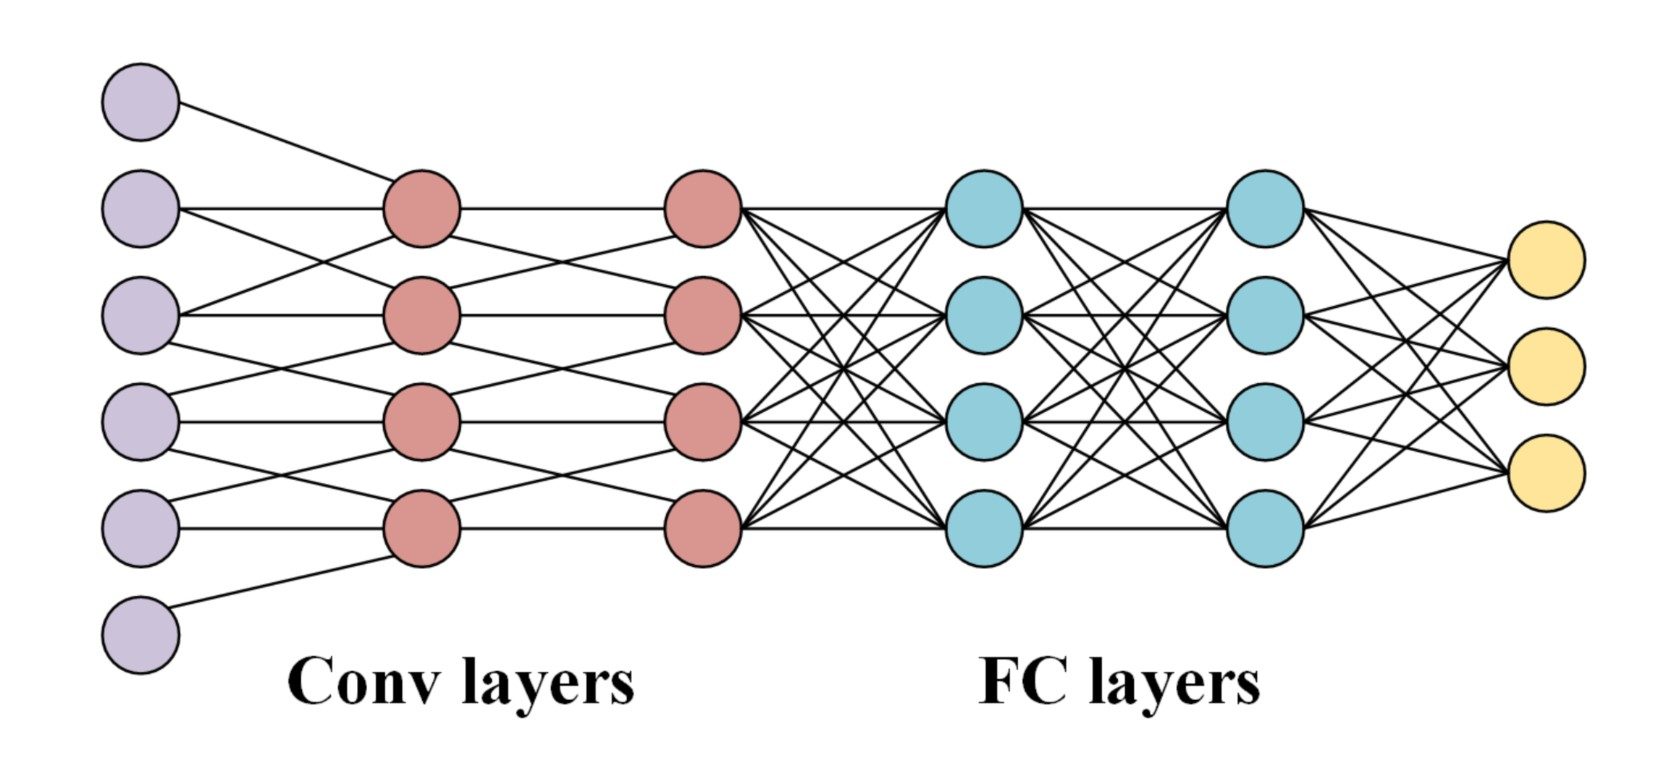
\includegraphics[width=0.8\textwidth]{Images/DataMining/CNNandFCLayers}
	\caption{CNN and FC layers \cite{Li:2021}.} \label{fig:CNNandFCLayers}
\end{figure}


Convolution is a crucial step for feature extraction. Convolution generates feature maps. To mitigate information loss at the border, padding enlarges the input with zero values. Stride is employed to control convolution density. Post-convolution, feature maps may lead to overfitting, necessitating pooling (max pooling or average pooling) for redundancy elimination. The overall CNN procedure is illustrated in Figure \ref{fig:ProcedureCNN}. The terms padding, stride, and pooling are explained as follows:

\begin{itemize}
	\item \textbf{Padding:} Padding involves adding extra border pixels to the input image before convolution. This is done by appending additional rows and columns of zero values around the image. The purpose of padding is to mitigate information loss at the borders during convolutional operations.
	
	\item \textbf{Stride:} Stride is the step size or the number of pixels by which the convolutional filter moves across the input image during the convolution operation. A larger stride reduces the spatial dimensions of the feature maps, leading to a more compact representation.
	
	\item \textbf{Pooling:} Pooling is a down-sampling operation applied after convolution. It reduces the spatial dimensions of the feature maps, helping to control the number of parameters in the network. Pooling is typically performed using operations such as max pooling or average pooling.
	
	\begin{itemize}
		\item \textbf{Max Pooling:} Max pooling is a specific pooling operation where, for each region of the feature map, the maximum value is taken. This helps retain the most significant information from that region, providing a form of spatial summarization.
		
		\item \textbf{Average Pooling:} Average pooling is another type of pooling operation where, for each region of the feature map, the average value is computed. This operation helps reduce the spatial dimensions while maintaining a smoother and less detailed representation.
	\end{itemize}
\end{itemize}


\begin{figure}[h!]
	\centering
	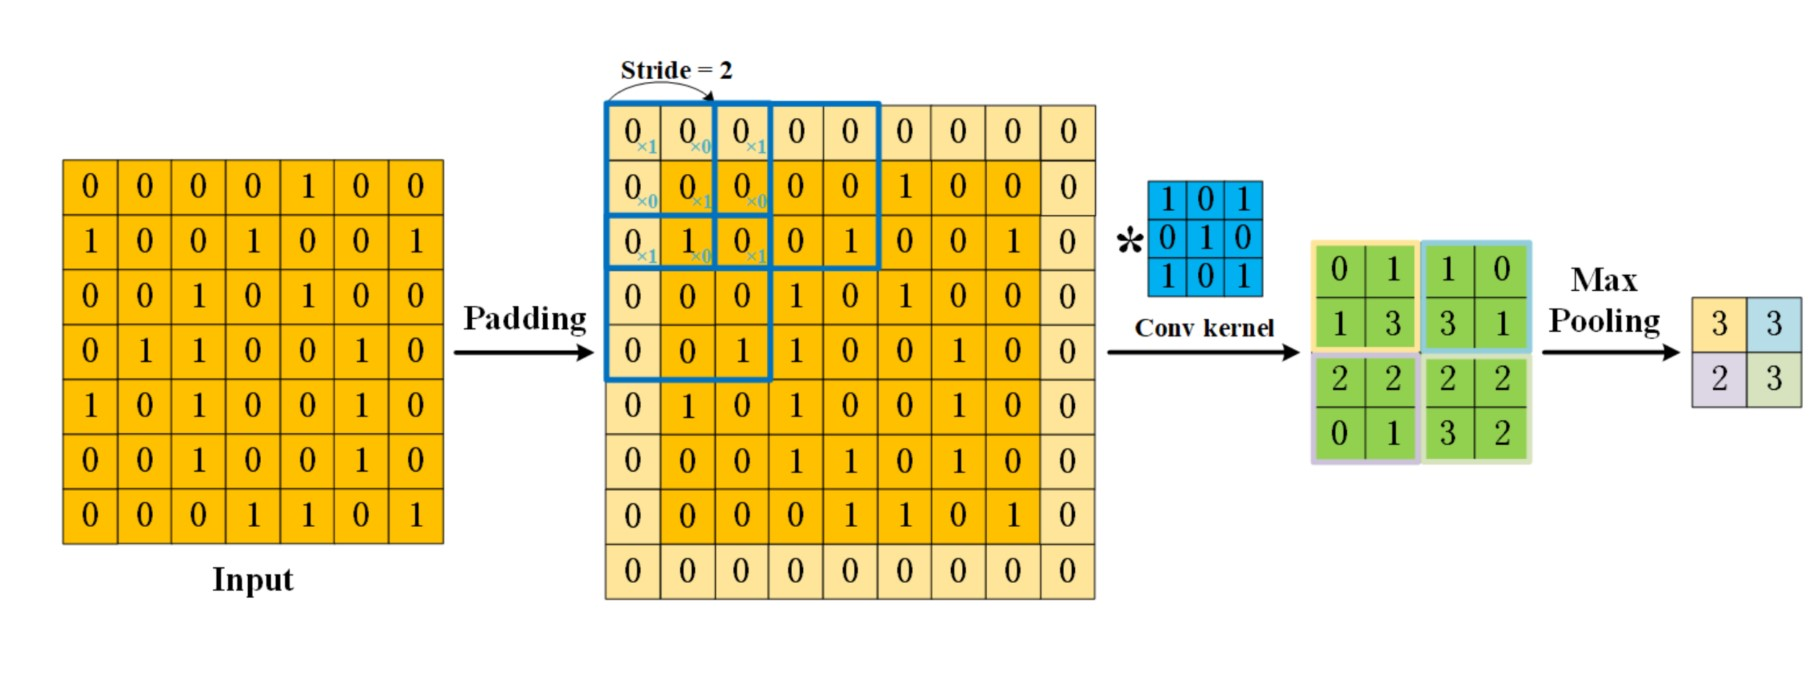
\includegraphics[width=0.8\textwidth]{Images/DataMining/ProcedureCNN}
	\caption{Procedure of a two-dimensional CNN \cite{Li:2021}.} \label{fig:ProcedureCNN}
\end{figure}

In the realm of Convolutional Neural Networks (CNNs), a variety of architectural variations exists, yet their fundamental components remain highly similar. Taking the renowned LeNet-5 as a case in point, it comprises three key layers: convolutional, pooling, and fully-connected layers. The primary purpose of the convolutional layer is to capture feature representations from the inputs \cite{Gu:2018}.

Illustrated in Figure \ref{subfig:LetNet5ArchitectureNetwork}, the convolutional layer is crafted from multiple convolution kernels responsible for computing distinct feature maps. Each neuron within a feature map establishes connections with a neighborhood of neurons in the preceding layer, known as the neuron's receptive field. The generation of a feature map involves convolving the input with a learned kernel, followed by the application of an element-wise nonlinear activation function to the results. It's important to note that each feature map is generated by sharing the kernel across all spatial locations of the input, thereby leveraging several diverse kernels for the complete set of feature maps.

\begin{figure}[h!]
	\centering
	
	\begin{subfigure}{0.65\textwidth}
		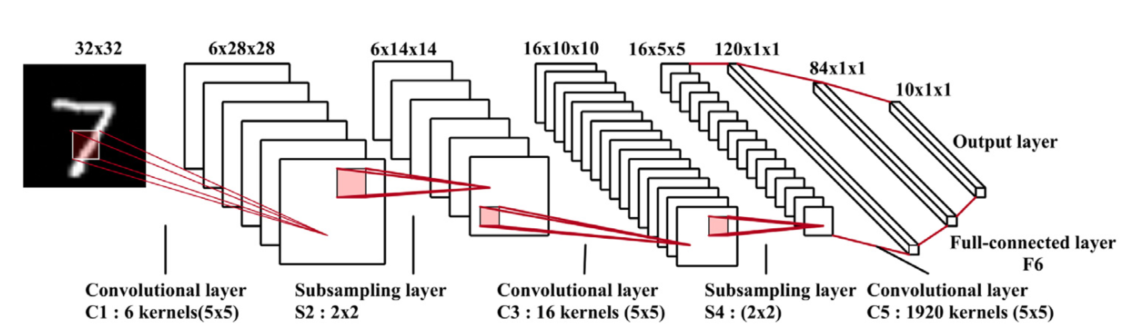
\includegraphics[width=\linewidth]{Images/DataMining/LetNet5ArchitectureNetwork}
		\caption{LetNet-5 network}    % \caption{} is kept to keep (a), (b), (c) etc. below each subfigure.
		\label{subfig:LetNet5ArchitectureNetwork}
	\end{subfigure}
	\hfill
	\begin{subfigure}{0.3\textwidth}
		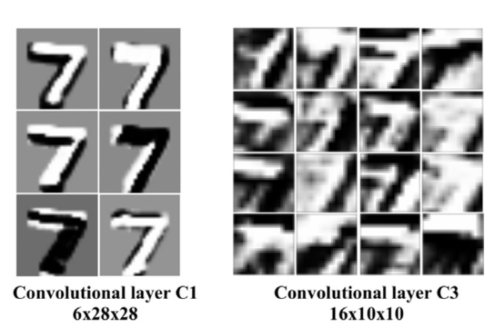
\includegraphics[width=\linewidth]{Images/DataMining/LetNet5ArchitectureLearnedFeatures}
		\caption{Learned features}    % \caption{} is kept to keep (a), (b), (c) etc. below each subfigure.
		\label{subfig:LetNet5ArchitectureLearnedFeatures}
	\end{subfigure}
	
	\caption{The architecture of the LeNet-5 network \cite{Gu:2018}. (\subref{subfig:LetNet5ArchitectureNetwork}) The architecture of the LeNet-5 network, renowned for its effectiveness in digit classification tasks. (\subref{subfig:LetNet5ArchitectureLearnedFeatures}) Displaying the features within the LeNet-5 network through visualizations, where each layer's feature maps are showcased in distinct blocks.}
	\label{fig:LetNet5Architecture}
\end{figure}

Mathematically, the feature value at location $(i, j)$ in the $k$th feature map of the $l$th layer (denoted as $z^l_{i,j,k}$) is computed by the expression:

\begin{equation}
	z^l_{i,j,k} = {\mathbf{w}^l_k}^T \mathbf{x}^l_{i,j} + b^l_k
\end{equation}

Where $\mathbf{w}^l_k$ and $ b^l_k$ represent the weight vector and bias term of the $k$th filter of the $l$th layer, while $\mathbf{x}^l_{i,j}$ is the input patch centered at location $(i, j)$ of the $l$th layer. The weight sharing mechanism, where the kernel generating the feature map is shared, offers advantages such as reducing model complexity and facilitating network training.

The activation function ($a(\cdot)$) introduces nonlinearity to the CNN, which is crucial for detecting nonlinear features in multi-layer networks. The activation value ($a_{l,i,j,k}$) of the convolutional feature $z_{l,i,j,k}$ is computed as:

\begin{equation}
	a^l_{i,j,k} = a(z^l_{i,j,k})
\end{equation}

Common activation functions include sigmoid, tanh, and ReLU. More information about activation functions is given in Subsection \ref{subsection:ActivationFunction}. The pooling layer, positioned between convolutional layers, aims to achieve shift-invariance by downsampling the feature maps' resolution. Each feature map in the pooling layer connects to its corresponding feature map in the preceding convolutional layer. The pooling operation, denoted as $\mathrm{pool}(\cdot)$, is applied to each feature map $a^l_{m,n,k}$ with:

\begin{equation}
	y^l_{i,j,k} = \mathrm{pool}(a^l_{m,n,k}), \forall (m, n) \in \mathcal{R}_{ij}
\end{equation}

Here, $\mathcal{R}_{ij}$ represents a local neighborhood around location $(i, j)$. Common pooling operations include average pooling and max pooling. The learned feature maps, as demonstrated in Figure \ref{subfig:LetNet5ArchitectureLearnedFeatures} for the digit 7, progressively capture hierarchical features, with early layers detecting low-level features like edges and curves, and subsequent layers encoding more abstract features.

Following the convolutional and pooling layers, one or more fully-connected layers may be present to perform high-level reasoning. These layers connect all neurons from the previous layer to every neuron in the current layer, generating global semantic information. Notably, a fully-connected layer can be replaced by a $1 \times 1$ convolution layer.

The final layer in CNNs is the output layer. For classification tasks, the softmax operator (see Subsection \ref{subsection:outputCNN}) is commonly employed. Alternatively, SVM can be combined with CNN features to address diverse classification tasks. Consider a set of $N$ desired input-output relationships represented as $\{(\mathbf{x}^{(n)}, \mathbf{y}^{(n)}); n \in [1, \ldots, N]\}$. The parameters of a CNN, denoted as $\mathbf{\theta}$, including weight vectors and bias terms, are optimized by minimizing an appropriate loss function defined for the specific task:

\begin{equation}
	\mathcal{L} = \frac{1}{N} \sum_{n=1}^{N} \ell(\mathbf{\theta}; \mathbf{y}^{(n)}, \mathbf{o}^{(n)})
\end{equation}

Here, $\mathcal{L}$ represents the loss function, which quantifies the discrepancy between the predicted output ($\mathbf{o}^{(n)}$) and the actual target label ($\mathbf{y}^{(n)}$) for $n$th input data point $\mathbf{x}^{(n)}$. The symbol $\mathbf{\theta}$ denotes all the parameters of the CNN, including weight vectors and bias terms. The function $\ell(\mathbf{\theta}; \mathbf{y}^{(n)}, \mathbf{o}^{(n)})$ is the individual loss for a specific data point, measuring the dissimilarity between the predicted output and the true label. The goal during training is to minimize the average loss over all data points, achieved through techniques such as stochastic gradient descent. Additional details about loss functions are available in Subsection \ref{subsection:LossFunction}.

The training of a CNN involves global optimization, with the aim of finding the best set of parameters by minimizing the loss function. Stochastic gradient descent emerges as a common solution for optimizing CNN networks, providing an effective means of iterative parameter adjustment. Optimizing is explained in the Subsection \ref{subsection:optimizer}. 

\subsection{Activation Function}
\label{subsection:ActivationFunction}

Convolutional Neural Networks (CNNs) leverage various activation functions to express intricate features \cite{Li:2021}. Functioning akin to the human brain's neuron model, the activation function serves as a unit determining the transmission of information to the next neuron. In a multilayer neural network, an activation function exists between two layers, structurally depicted in Figure \ref{fig:activationFunctionStructure}.

In Figure \ref{fig:activationFunctionStructure}, $x_i$ denotes input features, $n$ features simultaneously input to neuron $j$, $w_{ij}$ represents connection weight between input feature $x_i$ and neuron $j$, $b_j$ is the internal state (bias) of neuron $j$, and $y_j$ is the neuron's output. The activation function, denoted as $f(·)$ , includes options like the sigmoid, tanh, rectified linear unit (ReLU), and others.

When no activation function or a linear function is used, the network output is a linear combination of inputs, limiting learning ability. Nonlinear activation functions, like sigmoid and tanh, are introduced to enhance the network's capability to fit data.

\begin{figure}[h!]
	\centering
	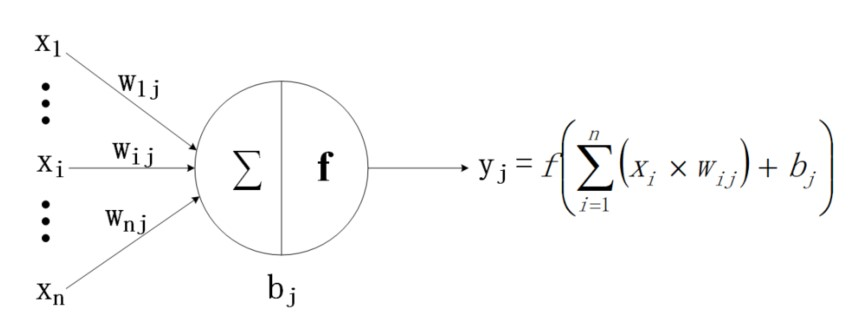
\includegraphics[width=0.6\textwidth]{Images/DataMining/activationFunctionStructure}
	\caption{Overall structure of an activation function \cite{Li:2021}.} \label{fig:activationFunctionStructure}
\end{figure}

Some of the well-known actiovatoion functions are shown in the Figure \ref{fig:activationFunctions}. The sigmoid function maps a real number to (0, 1), suitable for binary classification. The tanh function maps to (-1, 1), aiding normalization. ReLU, with its advantages in learning speed, is preferred in deep networks. Leaky ReLU and PReLU address limitations of ReLU, reducing neuron inactivation. ELU improves convergence by having a negative output average.

Swish, proposed by Google, and mish, a novel activation function, demonstrate improved performance compared to ReLU and Swish in deeper models across diverse datasets. mish, in particular, exhibits superior gradient flow, accuracy, and generalization properties. Experimental results consistently support the effectiveness of Mish across standard architectures.

\begin{figure}[h!]
	\centering
	
	\begin{subfigure}{0.22\textwidth}
		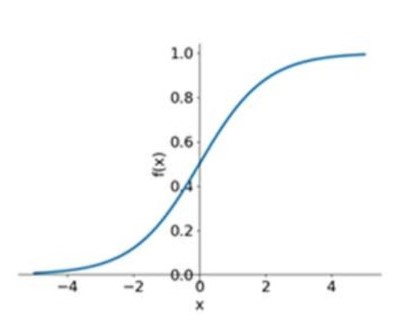
\includegraphics[width=\linewidth]{Images/DataMining/SigmoidFunction}
		\caption{}    % \caption{} is kept to keep (a), (b), (c) etc. below each subfigure.
		\label{subfig:Sigmoid}
	\end{subfigure}
	\hfill
	\begin{subfigure}{0.22\textwidth}
		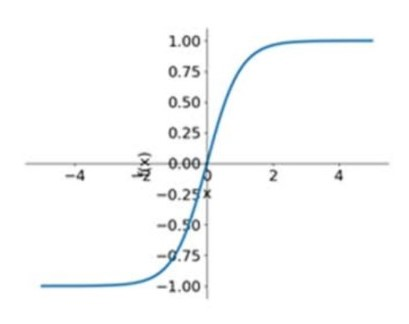
\includegraphics[width=\linewidth]{Images/DataMining/TanhFunction}
		\caption{}    % \caption{} is kept to keep (a), (b), (c) etc. below each subfigure.
		\label{subfig:Tanh}
	\end{subfigure}
	\hfill
	\begin{subfigure}{0.22\textwidth}
		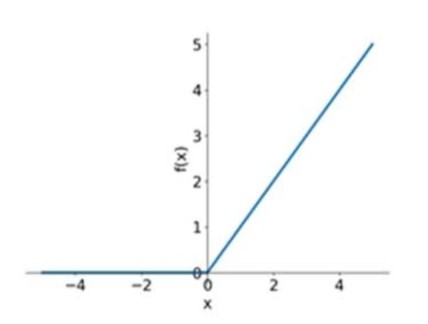
\includegraphics[width=\linewidth]{Images/DataMining/ReLUFunction}
		\caption{}    % \caption{} is kept to keep (a), (b), (c) etc. below each subfigure.
		\label{subfig:ReLU}
	\end{subfigure}
	\hfill
	\begin{subfigure}{0.22\textwidth}
		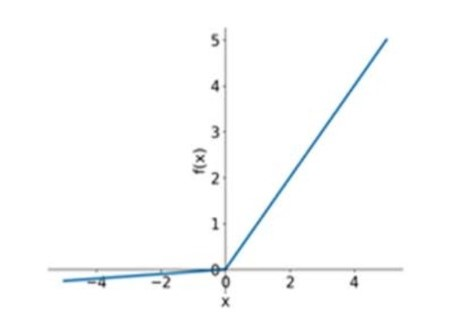
\includegraphics[width=\linewidth]{Images/DataMining/LeakyReLUFunction}
		\caption{}    % \caption{} is kept to keep (a), (b), (c) etc. below each subfigure.
		\label{subfig:LeakyReLU}
	\end{subfigure}
	
	\medskip
	
	\begin{subfigure}{0.22\textwidth}
		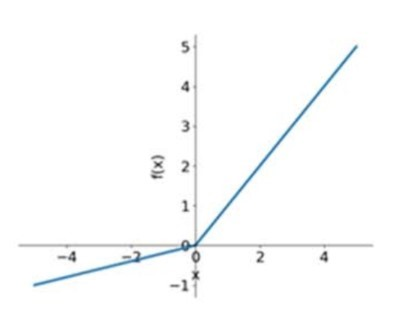
\includegraphics[width=\linewidth]{Images/DataMining/PReLUFunction}
		\caption{}    % \caption{} is kept to keep (a), (b), (c) etc. below each subfigure.
		\label{subfig:PReLU}
	\end{subfigure}
	\hfill
	\begin{subfigure}{0.22\textwidth}
		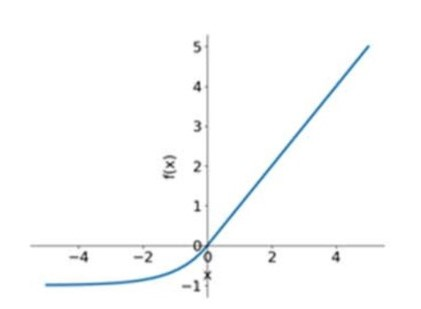
\includegraphics[width=\linewidth]{Images/DataMining/ELUFunction}
		\caption{}    % \caption{} is kept to keep (a), (b), (c) etc. below each subfigure.
		\label{subfig:ELU}
	\end{subfigure}
	\hfill
	\begin{subfigure}{0.22\textwidth}
		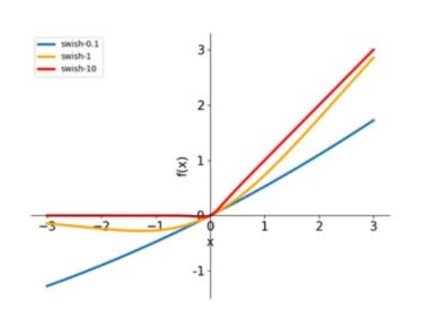
\includegraphics[width=\linewidth]{Images/DataMining/SwishFunctions}
		\caption{}    % \caption{} is kept to keep (a), (b), (c) etc. below each subfigure.
		\label{subfig:Swish}
	\end{subfigure}
	\hfill
	\begin{subfigure}{0.22\textwidth}
		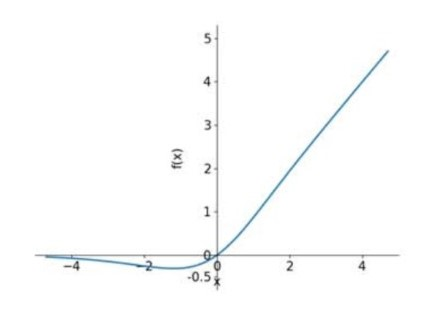
\includegraphics[width=\linewidth]{Images/DataMining/MishFunction}
		\caption{}    % \caption{} is kept to keep (a), (b), (c) etc. below each subfigure.
		\label{subfig:Mish}
	\end{subfigure}
	
	\caption{Diagrams of activation functions \cite{Li:2021}.  (\subref{subfig:Sigmoid}) Sigmoid function.  (\subref{subfig:Tanh}) Tanh function. (\subref{subfig:ReLU}) ReLU function. (\subref{subfig:LeakyReLU}) Leaky ReLU function. (\subref{subfig:PReLU}) PReLU function. (\subref{subfig:ELU}) ELU function.  (\subref{subfig:Swish}) Swish function. (\subref{subfig:Mish}) Mish function.}
	\label{fig:activationFunctions}
\end{figure}

\subsubsection{Guidelines for Activation Function Selection}

\begin{enumerate}
	\item For binary classification tasks, employ the sigmoid function in the last layer; for multiclassification, opt for the softmax function.
	\item Exercise caution with sigmoid and tanh functions due to potential gradient vanishing issues. Preferably, in hidden layers, consider ReLU or leaky ReLU for improved performance.
	\item When uncertain about the suitable activation function, consider experimenting with ReLU or leaky ReLU as reliable starting points.
	\item In cases where numerous neurons become inactive during training, explore alternatives like leaky ReLU, PReLU, or similar activation functions to address the issue.
	\item To expedite training, set the negative slope in leaky ReLU to 0.02, mitigating potential challenges associated with a slow convergence rate.
\end{enumerate}


\subsection{Loss Function}
\label{subsection:LossFunction}

The loss function, crucial in calculating the disparity between predicted and actual values, serves as a learning criterion for optimization in CNNs. It plays a key role in regression and classification problems, aiming to minimize the loss. Commonly used loss functions include Mean Absolute Error (MAE), Mean Square Error (MSE), and Cross Entropy \cite{Li:2021}.

\subsubsection{Loss Function for Regression}
In CNNs, MAE or MSE is commonly used for regression problems. MAE computes the mean absolute error, providing robustness to outliers. On the other hand, MSE calculates the mean of square errors, enabling controlled update rates. Choosing between them depends on the presence of outliers in the training set.

\subsubsection{Loss Function for Classification}
Various loss functions are employed in CNNs for classification tasks. The widely used cross entropy loss evaluates the difference between predicted probability distributions and actual distributions. While effective, it has limitations, focusing solely on classification correctness and neglecting factors like compactness within classes and margins between different classes.

\begin{itemize}
	\item \textbf{Contrastive Loss:}
	Enlarges distance between different categories and minimizes distance within the same categories, often used in dimensionality reduction for face recognition.
	
	\item \textbf{Triplet Loss:}
	Introduced for better face embeddings, minimizes the distance between anchor and positive images while increasing the distance to negative ones. Useful in fine-grained classification at the individual level.
	
	\item \textbf{Center Loss:}
	An improvement upon cross entropy, focuses on the uniformity of distribution within the same class by minimizing intraclass differences.
\end{itemize}

These diverse loss functions offer flexibility and cater to specific challenges encountered in regression and classification tasks within CNNs.

\subsubsection{Guidelines for Loss Function Selection}

\begin{enumerate}
	\item For regression challenges in CNN models, viable choices for the loss function include L1 loss or L2 loss.
	
	\item When confronted with classification tasks, opt for a suitable loss function from the available options.
	
	\item Cross entropy loss stands out as a prevalent choice, frequently employed in CNN models featuring a softmax layer at the conclusion.
	
	\item Addressing concerns regarding compactness within a class or the margin between different classes necessitates considering enhancements based on cross entropy loss. Examples include center loss and large-margin softmax loss.
	
	\item The choice of a loss function in CNNs should align with the specific application scenario. For instance, in face recognition applications, contrastive loss and triplet loss have emerged as commonly utilized options.
\end{enumerate}

\subsection{Optimizer}
\label{subsection:optimizer}

In CNNs, optimization of nonconvex functions is crucial, often necessitating optimizers to efficiently minimize the loss function within a reasonable timeframe \cite{Li:2021}. Nonconvex functions exhibit intricate landscapes with multiple local optima, making their optimization challenging. These functions lack the convex property, where any line segment connecting two points lies entirely within the function's domain, complicating the search for the global minimum.

Common optimization algorithms include momentum, Root-mean-square prop (RMSprop), adaptive moment estimation (Adam), etc.

\subsubsection{Gradient Descent}

Three gradient descent methods for training CNN models are batch gradient descent (BGD), stochastic gradient descent (SGD), and mini-batch gradient descent (MBGD).

\begin{itemize}
	\item BGD is slow due to calculating the average gradient of the entire batch, making it impractical for large datasets or in-memory constraints.
	\item SGD, using one sample per update, is suitable for online learning but prone to high variance and oscillations.
	\item MBGD, a popular choice, combines advantages of BGD and SGD, efficiently using a small batch to stabilize convergence.
\end{itemize}

\subsubsection{Gradient Descent Optimization Algorithms}

Effective algorithms built on MBGD include:

\begin{itemize}
	\item Momentum algorithm simulates physical momentum, preventing oscillations for faster convergence.
	\item Nesterov accelerated gradient (NAG) enhances momentum algorithm predictability to slow down before positive slopes.
	\item Adagrad adapts the learning rate to parameters, suitable for sparse data.
	\item Adadelta limits the monotonically decreasing learning rate of Adagrad.
	\item RMSprop addresses diminishing learning rate issues in Adagrad.
	\item Adam combines momentum with RMSprop, proving effective in various CNN structures.
	\item Other variants like AdaMax, Nadam, and AMSGrad offer improvements and constraints.
\end{itemize}

\subsubsection{Guidelines for Optimizer Selection:}

\begin{enumerate}
	\item Utilize Mini-Batch Gradient Descent (MBGD) to strike a balance between Batch Gradient Descent (BGD) and Stochastic Gradient Descent (SGD), considering both computing cost and the accuracy of each update.
	
	\item Optimizer performance is intricately linked to data distribution. Adhering to the No Free Lunch Theorem, no single optimizer universally outperforms others in all scenarios. A prudent approach involves selecting optimizers based on their unique characteristics.
	
	\item In instances of excessive oscillation or divergence, it is advisable to contemplate reducing the learning rate to address these issues.
\end{enumerate}

\section{Applications}

The utilization of Convolutional Neural Networks (CNN) in computer vision has made possible achievements that were once deemed impossible over the past centuries. These accomplishments include facial recognition, autonomous vehicles, self-service supermarkets, and intelligent medical treatments \cite{Li:2021}.

\subsubsection{1-D CNN Applications}

\begin{enumerate}
	\item \textbf{Time Series Prediction:}
	\begin{itemize}
		\item Applied to predict time series data, such as electrocardiogram (ECG) time series, weather forecast, and traffic flow prediction.
		\item Example: Prediction of atrial fibrillation using short-term ECG data.
	\end{itemize}
	
	\item \textbf{Signal Identification:}
	\begin{itemize}
		\item Used for discriminating input signals based on features learned from training data.
		\item Applications include ECG signal identification, structural damage identification, and system fault identification.
	\end{itemize}
\end{enumerate}

\subsubsection{2-D CNN Applications}

\textbf{keyword spotting:} One of the key applications of artificial neural networks in the consumer domain is found in the realm of digital assistants, particularly in the area of automatic speech recognition. By employing automatic speech recognition, digital assistants empower users to effortlessly control devices through spoken commands. While automatic speech recognition has been in existence since the 1980s, utilizing methods such as Hidden Markov models and Gaussian mixture models, it was not until 2012 that artificial neural networks were introduced to address this challenge. This marked a significant enhancement in user experience and played a pivotal role in boosting the widespread adoption of digital assistants. Effectively managing audio data streams through continuous processing by an artificial neural network becomes challenging when dealing with multiple users. Additionally, the persistent recording of audio data raises valid privacy and security concerns. As a result, the device needs to identify a pre-defined keyword before transmitting audio data to the server, a procedure commonly known as keyword spotting \cite{Bushur:2023}.

Other 2-D applications of CNNs are:

\begin{enumerate}
	\item \textbf{Image Classification:}
	\begin{itemize}
		\item Task of classifying images into categories.
		\item Used in medical image classification, traffic scenes related classification, etc.
		\item Example: Custom CNN for the classification of interstitial lung disease.
	\end{itemize}
	
	\item \textbf{Object Detection:}
	\begin{itemize}
		\item Involves identifying objects within images and marking them with bounding boxes.
		\item Two-stage approaches like R-CNN, fast R-CNN, and faster R-CNN, as well as one-stage approaches like YOLO, are discussed.
		\item Applications in detecting objects in images or videos.
	\end{itemize}
	
	\item \textbf{Image Segmentation:}
	\begin{itemize}
		\item Divides an image into different areas and marks the boundaries of semantic entities.
		\item Examples include U-Net for medical image segmentation and Panoptic segmentation.
		\item Applications in medical image segmentation and semantic segmentation.
	\end{itemize}
	
	\item \textbf{Face Recognition:}
	\begin{itemize}
		\item A biometric identification technique based on facial features.
		\item Evolution from DeepFace to more recent approaches like FaceNet, VGGFace, etc.
		\item Different loss functions, such as triplet loss, are employed for training.
	\end{itemize}
\end{enumerate}

\subsubsection{Multidimensional CNN Applications}

\begin{enumerate}
	\item \textbf{Human Action Recognition:}
	\begin{itemize}
		\item Involves recognizing human actions in videos.
		\item 3D CNNs used to extract features, and integration with 2D CNN features is discussed.
	\end{itemize}
	
	\item \textbf{Object Recognition/Detection in 3D:}
	\begin{itemize}
		\item Applications like object detection of RGBD images using 3D ShapeNet and VoxNet for 3D object recognition.
		\item Detection of high-dimensional images like X-rays and CT images using 3D CNN.
	\end{itemize}
\end{enumerate}


\section{Why CNN is relevant}

Choosing a Convolutional Neural Network (CNN) for speech recognition is justified by the nature of the input data—spectrograms (see Section \ref{subsection:InputDataSpeech}). Since spectrograms are two-dimensional arrays, a neural network must adeptly handle multidimensional tensors. CNNs, designed for precisely this purpose, excel in extracting features from relationships between adjacent values in such data \cite{Warden:2019}.

CNNs, commonly associated with image processing, excel at learning hierarchical features, starting from simple elements like lines or edges and progressing to complex structures like eyes or ears. Importantly, their adaptability extends beyond images, making them well-suited for any multidimensional vector input.

Given that spectrogram data shares similarities with images as two-dimensional grids, CNNs are a natural fit. Their ability to capture relationships in a two-dimensional space aligns perfectly with the structure of spectrograms, making CNNs an effective choice for speech recognition, facilitating the extraction of meaningful features from the input data.

\section{Hyperparameters}

From tuning activation functions, loss functions, and optimizers to adjusting various other hyperparameters, the impact on model performance is substantial. It is well-established that there is no universally fixed set of hyperparameters that guarantees optimal solutions at all times. Consequently, relying on a combination of experience and established guidelines becomes crucial when navigating the intricate process of hyperparameter tuning \cite{Li:2021}.

\begin{itemize}
	\item \textbf{Learning Rate:} Refers to the step size of updating network weights. It can be constant or variable. It should be set in an appropriate range to balance convergence speed and stability.
	
	\item \textbf{Epoch:} The number of times the whole training set is input to the neural network for training. Should be adjusted based on the gap between training set and validation set accuracy to avoid underfitting or overfitting.
	
	\item \textbf{Mini-Batch Size:} The number of samples sent to the model in each training iteration. Too small or too large batch sizes can affect convergence and stability. Often set to dozens to hundreds, usually a power of 2 for \ac{gpu} performance optimization.
	
	\item \textbf{Number of Conv Layers:} Determines the depth of the network and its ability to capture different-level features. More layers generally allow the representation of more complex features but can be harder to train.
	
	\item \textbf{Conv Kernel Size:} The size of convolution kernels in each layer. The smaller the kernel, the fewer parameters and computational complexity. Commonly used sizes include 3x3, 1x1, 1xn, and nx1.
	
	\item \textbf{Number of Filters (Kernels):} The number of filters in each convolutional layer, determining the depth and capacity of the network. Often increases in deeper layers.
	
	\item \textbf{Activation Function:} Introduces non-linearity to the network. Common choices include ReLU, Sigmoid, and Tanh. The choice depends on the nature of the problem and data characteristics.
\end{itemize}


\section{Requirements}

\begin{itemize}
	\item \textbf{Model Size and Complexity:} Design a compact and computationally efficient CNN model that strikes a balance between accuracy and size, considering the limited memory and processing power of Arduino Nano.
	
	\item \textbf{Input Format:} Tailor the CNN to handle the specific format and characteristics of audio input suitable for Arduino Nano's limited input data capabilities.
	
	\item \textbf{Real-time Processing:} Optimize the CNN for real-time processing to ensure timely responses for speech recognition in the dynamic scenarios of Arduino Nano.
	
	\item \textbf{Energy Efficiency:} Develop an energy-efficient CNN that minimizes power consumption during inference without compromising performance, acknowledging the limited power resources on Arduino Nano.
	
	\item \textbf{Output Interface:} Align the CNN's output format with the device's capabilities to facilitate seamless integration with Arduino Nano, recognizing and utilizing its limited output capabilities.
	
	\item \textbf{Noise Robustness:} Incorporate features or preprocessing steps in the CNN to enhance noise robustness, adapting to different acoustic environments and addressing potential variability in environmental conditions.
	
	\item \textbf{Inference Speed:} Optimize the CNN for fast inference to ensure prompt recognition of spoken commands, considering the limited processing speed of Arduino Nano.
	
	\item \textbf{Training Considerations:} Design the CNN to be trainable with a manageable amount of data, considering the limited availability of training data for Arduino Nano, and address the specific nuances of the intended speech recognition application.
	
	\item \textbf{Postprocessing Techniques:} Implement postprocessing methods, such as score averaging or consensus-based recognition, to refine and enhance the accuracy of speech recognition in real-world scenarios with uncertainties.
	
	\item \textbf{Compatibility:} Ensure that the CNN model architecture and parameters are compatible with the hardware specifications of Arduino Nano, ensuring seamless integration and optimal performance on the device.
\end{itemize}


\section{Input}

In the realm of Convolutional Neural Networks (CNNs), understanding the intricacies of input data is paramount for effective model design and training. Here, the structure of input data is represented, emphasizing its role as a multi-dimensional array—commonly known as a tensor.

\subsection{Input Data Specifications}


\subsubsection{Dimensions for Image Data}

The input data in a Convolutional Neural Network (CNN) is fundamentally structured as a multi-dimensional array, commonly referred to as a tensor. This tensor represents the raw input to the neural network and is pivotal for subsequent feature extraction and hierarchical representation learning.

\subsubsection{Input Shape Specifications}

For image data, the tensor dimensions typically encompass the height, width, and channels of the image. In the context of color images using the RGB color space, the shape of the tensor is commonly denoted as (height, width, 3). Here, "height" and "width" correspond to the spatial dimensions of the image, and "3" indicates the three color channels (Red, Green, Blue). For example, if you have an image with dimensions $100 \times 100$ pixels, the RGB representation would be a $100 \times 100 \times 3$ matrix, where each element corresponds to the intensity of the respective color channel at that pixel.

Grayscale images, on the other hand, have only one channel. Each pixel in a grayscale image is represented by a single value indicating the intensity of brightness. The range of intensity values depends on the bit depth; for an 8-bit image, values typically range from 0 (black) to 255 (white). The matrix representing a grayscale image would be a 2D matrix, where each element represents the intensity of a pixel. In the Figure \ref{fig:DigitalImage} the digital presentation of the number "4" is presented. Note that the pixel values are normalized to be between 0 and 1, with 0 representing the black color and 1 representing the white color pixel value. 

\begin{figure}[h!]
	\centering
	
	\begin{subfigure}{0.45\textwidth}
		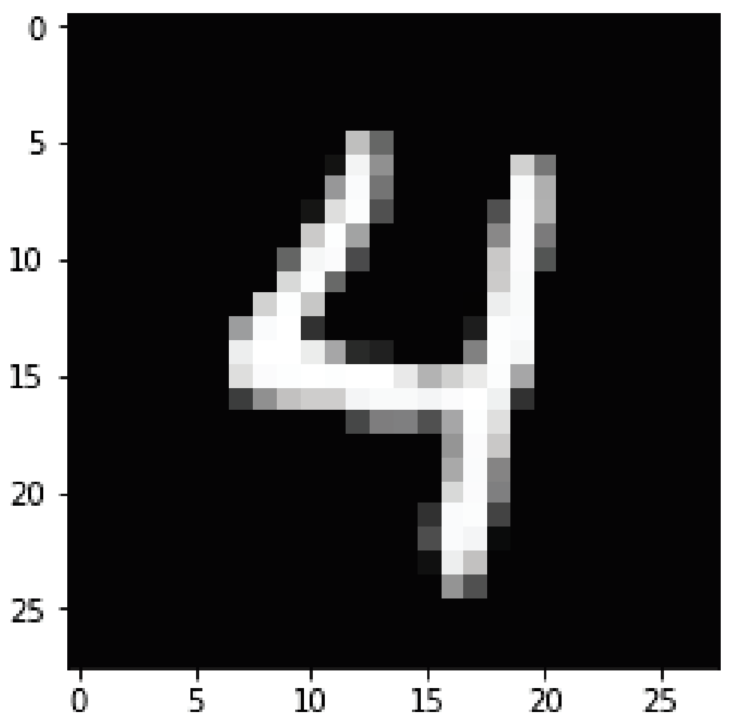
\includegraphics[width=\linewidth]{Images/DataMining/DigitalImage}
		\caption{}    % \caption{} is kept to keep (a), (b), (c) etc. below each subfigure.
		\label{subfig:DigitalImage}
	\end{subfigure}
	\hfill
	\begin{subfigure}{0.45\textwidth}
		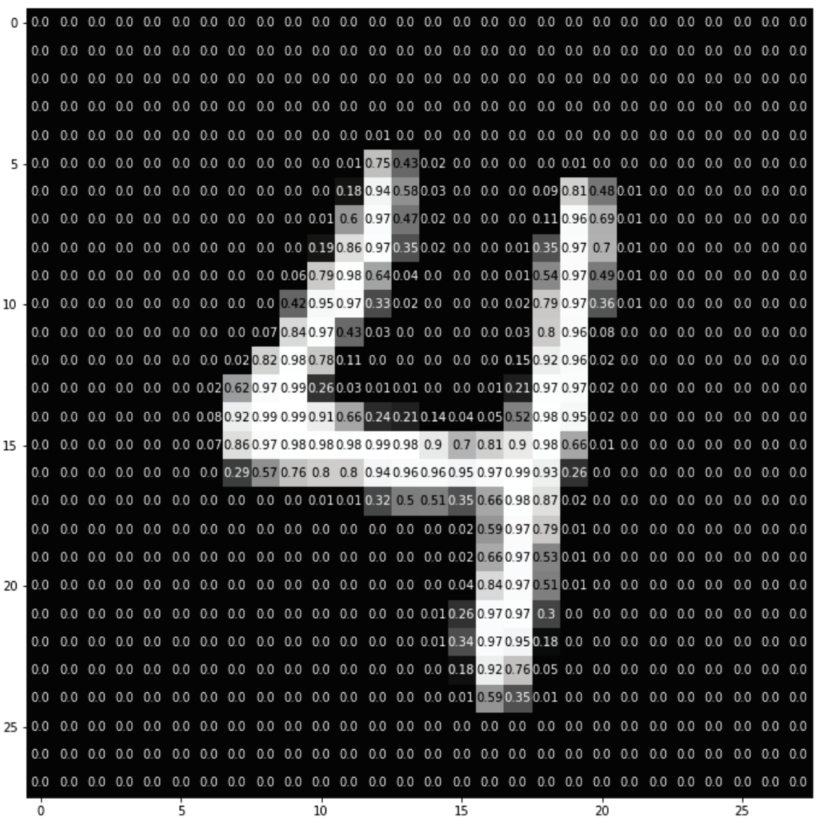
\includegraphics[width=\linewidth]{Images/DataMining/DigitalImagePixelValues}
		\caption{}    % \caption{} is kept to keep (a), (b), (c) etc. below each subfigure.
		\label{subfig:DigitalImagePixelValues}
	\end{subfigure}
	
	\caption{Digital presentation of an image \cite{Sewak:2018}. (\subref{subfig:DigitalImage}) Digital presentation of the number "4." (\subref{subfig:DigitalImagePixelValues}) Normalized pixel values of the number "4."}
	\label{fig:DigitalImage}
\end{figure}

\subsubsection{Normalization (Optional)}

Normalization layers, such as Batch Normalization, can be optionally employed within the input layer to facilitate stable training. Normalization involves adjusting the input values to a layer, ensuring that they fall within a standardized range. This can enhance convergence during training and mitigate issues related to vanishing or exploding gradients.


\subsection{Input Data for Speech Recognition Applications}
\label{subsection:InputDataSpeech}

It's important to note that he model does not process raw audio sample data; instead, it operates on spectrograms \cite{Warden:2019}; two dimensional arrays comprised of slices of frequency information, each derived from distinct time windows. Figure \ref{subfig:SpectralYes} visually depicts a spectrogram generated from a one-second audio clip of the word "yes," while Figure \ref{subfig:SpectralsNo} illustrates the same for the word "no."

\begin{figure}[h!]
	\centering
	
	\begin{subfigure}{0.45\textwidth}
		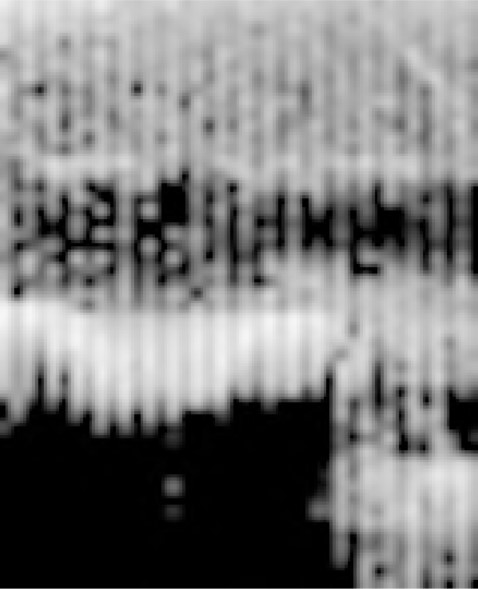
\includegraphics[width=\linewidth]{Images/DataMining/SpectrogramYes.jpg}
		\caption{}    % \caption{} is kept to keep (a), (b), (c) etc. below each subfigure.
		\label{subfig:SpectralYes}
	\end{subfigure}
	\hfill
	\begin{subfigure}{0.45\textwidth}
		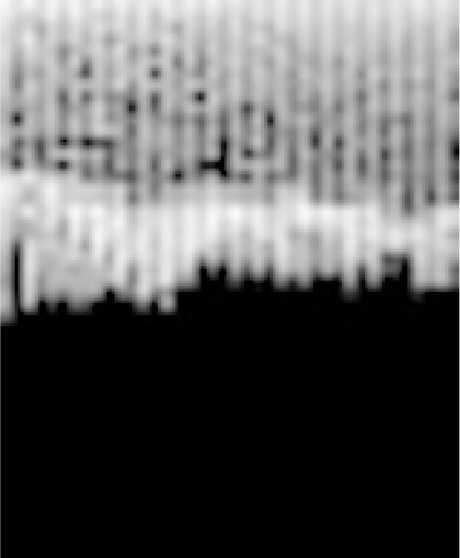
\includegraphics[width=\linewidth]{Images/DataMining/SpectrogramNo.jpg}
		\caption{}    % \caption{} is kept to keep (a), (b), (c) etc. below each subfigure.
		\label{subfig:SpectralsNo}
	\end{subfigure}
	
	\caption{Spectral representations of "yes" and "no" \cite{Warden:2019}. (\subref{subfig:SpectralYes}) Spectral representation of the word "yes." (\subref{subfig:SpectralsNo}) Spectral representation of the word "no."}
	\label{fig:SpectralYesNoCombined}
\end{figure}

By isolating frequency information during preprocessing, we simplify the model's training. It sidesteps the need to decipher raw audio data and instead operates with a higher-layer abstraction, distilling the most pertinent information. As a spectrogram is a two-dimensional array, it is inputted into the model as a 2D tensor.

Figure \ref{subfig:SpectralYes} depicts the input fed into the neural network, represented as a 2D array with a single channel, resembling a monochrome image. Working with 16 KHz audio sample data, the goal is to employ "feature generation" to transform a challenging input format (16,000 numerical values per second of audio) into a more machine-friendly representation. While machine vision often deals easily with images, domains like audio and natural language processing commonly require preprocessing before feeding data into a model.

To understand why preprocessing aids model comprehension, examine the original raw representations of audio recordings in Figures \ref{subfig:WaveformYesFirst} through \ref{subfig:WaveformNoSecond}. Without labels, distinguishing identical words is challenging. In contrast, Figures \ref{subfig:SpectrogramYesFirst} through \ref{subfig:SpectrogramNoSecond} demonstrate the spectrograms of the same recordings. Spectrograms, compared to raw waveforms, make differences more discernible, facilitating model interpretation.

\begin{figure}[h!]
	\centering
	
	\begin{subfigure}{0.45\textwidth}
		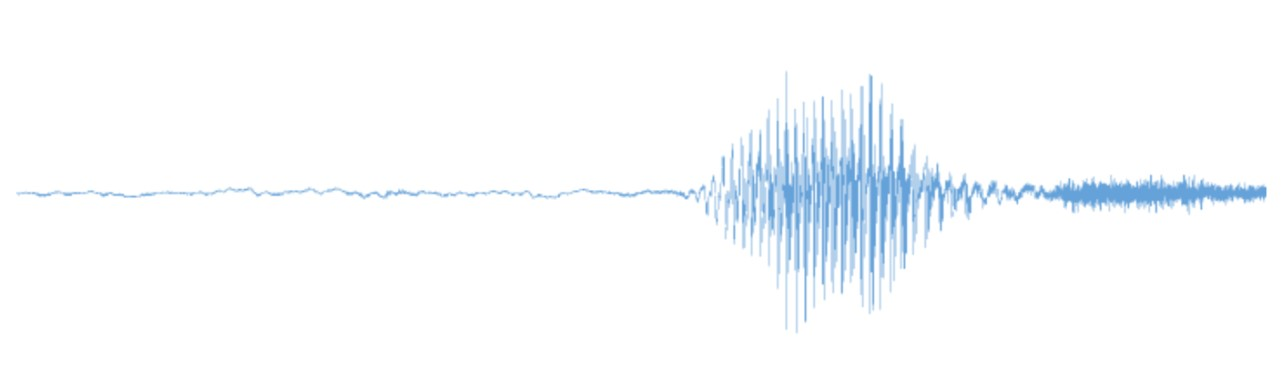
\includegraphics[width=\linewidth]{Images/DataMining/WaveformYesFirst.jpg}
		\caption{}    % \caption{} is kept to keep (a), (b), (c) etc. below each subfigure.
		\label{subfig:WaveformYesFirst}
	\end{subfigure}
	\hfill
	\begin{subfigure}{0.45\textwidth}
		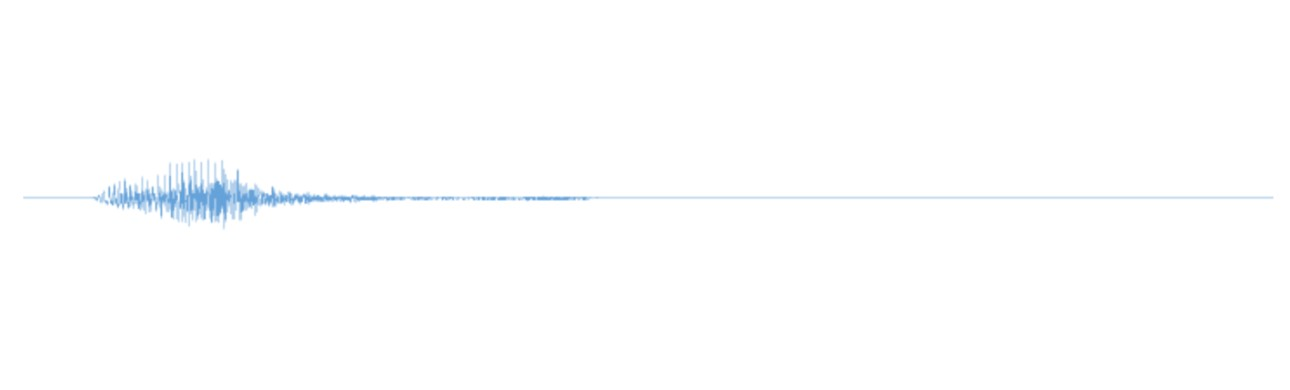
\includegraphics[width=\linewidth]{Images/DataMining/WaveformYesSecond.jpg}
		\caption{}    % \caption{} is kept to keep (a), (b), (c) etc. below each subfigure.
		\label{subfig:WaveformYesSecond}
	\end{subfigure}
	
	\medskip 
	
	\begin{subfigure}{0.45\textwidth}
		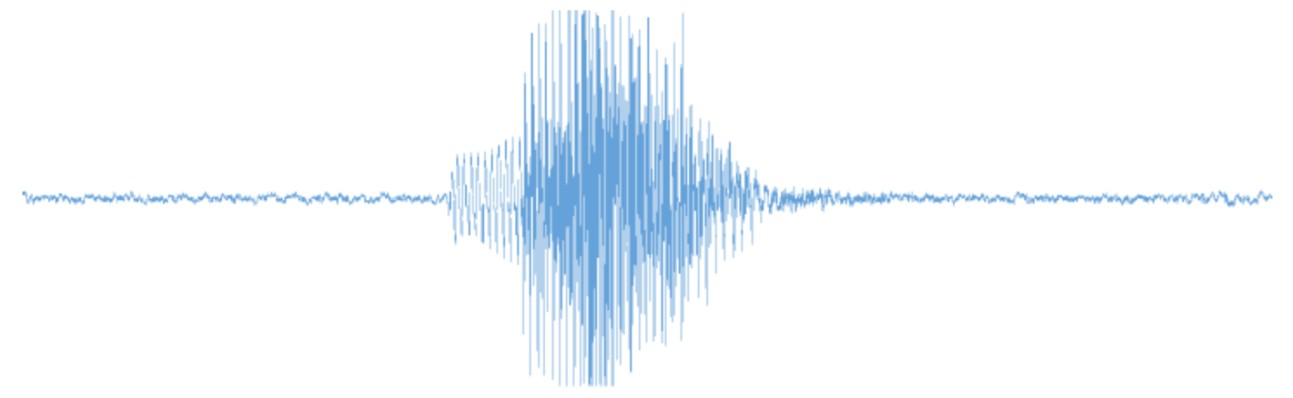
\includegraphics[width=\linewidth]{Images/DataMining/WaveformNoFirst.jpg}
		\caption{}    % \caption{} is kept to keep (a), (b), (c) etc. below each subfigure.
		\label{subfig:WaveformNoFirst}
	\end{subfigure}
	\hfill
	\begin{subfigure}{0.45\textwidth}
		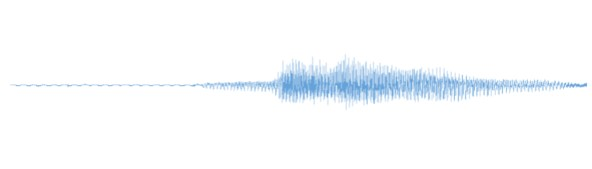
\includegraphics[width=\linewidth]{Images/DataMining/WaveformNoSecond.jpg}
		\caption{}    % \caption{} is kept to keep (a), (b), (c) etc. below each subfigure.
		\label{subfig:WaveformNoSecond}
	\end{subfigure}
	
	\caption{Audio waveforms of "yes" and "no" \cite{Warden:2019}. (\subref{subfig:WaveformYesFirst}) "yes" audio waveform. (\subref{subfig:WaveformYesSecond}) Another "yes" audio waveform. (\subref{subfig:WaveformNoFirst}) "no" audio waveform. (\subref{subfig:WaveformNoSecond}) Another "no" audio waveform.}
	\label{fig:audioWaveforms}
\end{figure}


\begin{figure}[h!]
	\centering
	
	\begin{subfigure}{0.45\textwidth}
		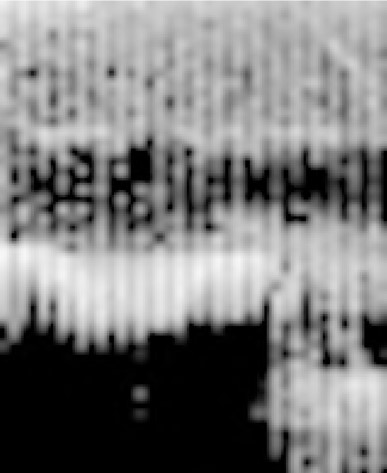
\includegraphics[width=\linewidth]{Images/DataMining/SpectrogramYesFirst.jpg}
		\caption{}    % \caption{} is kept to keep (a), (b), (c) etc. below each subfigure.
		\label{subfig:SpectrogramYesFirst}
	\end{subfigure}
	\hfill
	\begin{subfigure}{0.45\textwidth}
		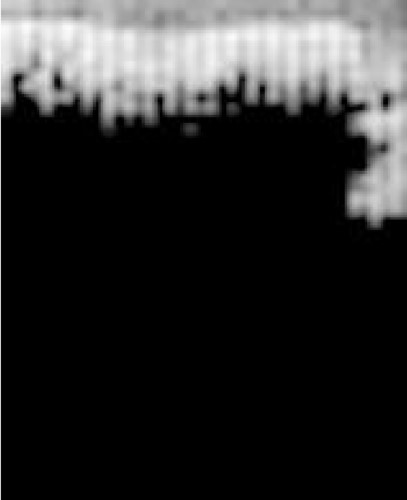
\includegraphics[width=\linewidth]{Images/DataMining/spectrogramYesSecond.jpg}
		\caption{}    % \caption{} is kept to keep (a), (b), (c) etc. below each subfigure.
		\label{subfig:SpectrogramYesSecond}
	\end{subfigure}
	
	\medskip 
	
	\begin{subfigure}{0.45\textwidth}
		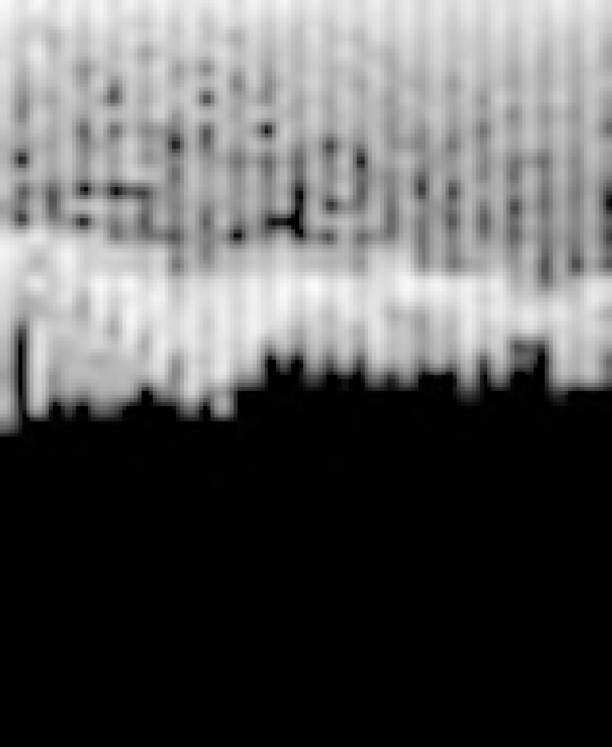
\includegraphics[width=\linewidth]{Images/DataMining/SpectrogramNoFirst.jpg}
		\caption{}    % \caption{} is kept to keep (a), (b), (c) etc. below each subfigure.
		\label{subfig:SpectrogramNoFirst}
	\end{subfigure}
	\hfill
	\begin{subfigure}{0.45\textwidth}
		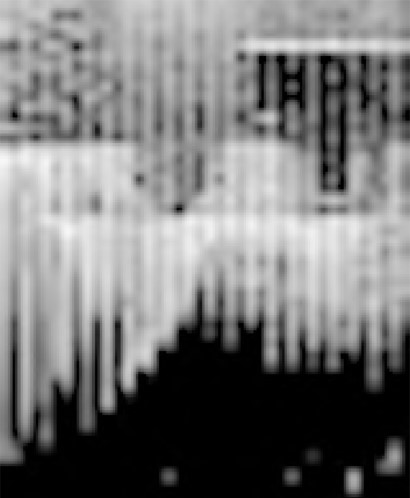
\includegraphics[width=\linewidth]{Images/DataMining/SpectrogramNoSecond.jpg}
		\caption{}    % \caption{} is kept to keep (a), (b), (c) etc. below each subfigure.
		\label{subfig:SpectrogramNoSecond}
	\end{subfigure}
	
	\caption{Audio Spectrograms of "yes" and "no" \cite{Warden:2019}. (\subref{subfig:SpectrogramYesFirst}) "yes" audio spectrogram (\subref{subfig:SpectrogramYesSecond}) Another "yes" audio spectrogram. (\subref{subfig:SpectrogramNoFirst}) "no" audio spectrogram. (\subref{subfig:SpectrogramNoSecond}) Another "no" audio spectrogram.}
	\label{fig:audioSpectrograms}
\end{figure}

Additionally, generated spectrograms are much smaller than raw sample data, with each containing 1,960 numeric values instead of 16,000 in the waveform. This summarization reduces the neural network's workload. While models like DeepMind's WaveNet \cite{Oord:2016} can handle raw data, they often entail more computation than the combination of a neural network with hand-engineered features, making the latter preferable for resource-constrained environments like embedded systems.

\subsection{How to Convert Audio to a Spectrogram}
\label{subsection:convertAudio}

The process of converting audio into a spectrogram involves creating a 2D array to represent an audio snippet, with each row reflecting a segment of the audio split into frequency buckets. This occurs in a loop, generating new features efficiently for the time elapsed since the last iteration \cite{Warden:2019}.

For each row, a segment of the audio undergoes fast Fourier transform (FFT) to analyze frequency distribution, resulting in condensed frequency information. The 2D array is formed by combining results from consecutive slices of the audio signal, ensuring continuity.

The decision on which slices to generate is based on time intervals between operations, optimizing computational efficiency. The loop retrieves audio samples for each new slice, and after processing, a comprehensive spectrogram is obtained. The subsequent steps involve using this spectrogram for inference with the model, and the results are interpreted for recognition.

In the Figure \ref{fig:audioProcessings} the diagram of audio samples being processed is shown. The process in this example involves converting audio into a spectrogram by analyzing one-second audio snippets in a loop. Each 30-millisecond audio segment undergoes a fast Fourier transform (FFT), producing an array of 256 frequency buckets, which are then averaged into 43 buckets to distill relevant frequency information. These steps are repeated for consecutive segments with a 20-millisecond overlap, ensuring continuity. The resulting frequency data forms a 2D array, representing the entire one-second audio sample.

\begin{figure}[h!]
	\centering
	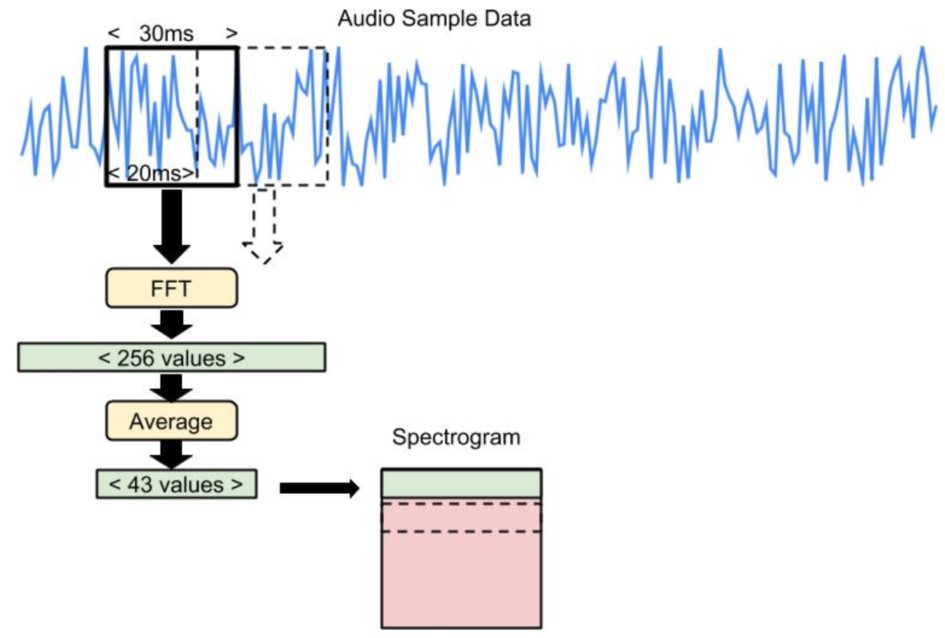
\includegraphics[width=0.8\textwidth]{Images/DataMining/audioProcessing.jpg}
	\caption{Diagram of the processing of audio samples \cite{Warden:2019}.} 
	\label{fig:audioProcessings}
\end{figure}


\section{Output}
\label{key}

In this section, the output of the CNN algorithm is explained. Initially, the output of the CNN for classification and regression tasks are explained in general terms. Subsequently, the output of the model for speech recognition applications is explained.

\subsection{The Output of the CNN Algorithm for Classification and Regression Tasks}

\subsubsection{Classification}

In a classification task, a Convolutional Neural Network (CNN) produces an output that represents a probability distribution over different classes. This is achieved through the use of a softmax activation function (explained later) in the final layer, ensuring that the output values signify probabilities. The class with the highest probability is then considered the predicted class.

\subsubsection{Regression}

In a regression task, the CNN output is a continuous numerical value. The network is designed to predict a specific numerical outcome, and the final layer often uses an activation function, such as linear, that allows for unbounded output. The training process involves minimizing the difference between the predicted value and the actual target value, as determined by the chosen loss function.

\subsection{Output of the Model for Speech Recognition Applications}
\label{subsection:outputCNN}

The CNN model in the case of speech recognition operates as a classifier, generating class probabilities as output. The final outcome of the model is determined by the output of the softmax (explained later) layer, resulting in, for example, four numbers corresponding to categories: "silence," "unknown," "yes," and "no" \cite{Warden:2019}. These numerical values represent the scores for each category, and the category with the highest score is the model's prediction, indicating the model's confidence in that prediction. For instance, if the model outputs \texttt{[10, 4, 231, 80]}, it predicts that the third category, "yes," is the most likely result with a score of 231. 

To avoid word recognition failure the model needs to run more frequently than once per second. Postprocessing methodologies are implemented to refine the model's predictions over time. A common approach involves averaging scores obtained from multiple runs, contributing to a more stable and reliable output. Recognition events are often triggered when there is a consensus of high scores for the same word within a condensed timeframe. This adaptive strategy enhances the robustness of the speech recognition system, allowing it to adapt to variations in speech patterns and environmental conditions.

Upon successful recognition, the command responder utilizes the device's output capabilities, such as flashing an LED or displaying information on an LCD screen. The model's output is structured with two dimensions, where the first is a wrapper and the second holds the probabilities for each class. This output format aligns with the requirements for our embedded hardware implementation on Arduino Nano 33 BLE Sense.

\subsubsection{The Softmax Function}

The softmax function is commonly used in Convolutional Neural Networks (CNNs) and other machine learning models, particularly in the output layer, to convert a vector of raw scores or logits into probabilities. It essentially normalizes the input values into a probability distribution that sums to 1 \cite{Sewak:2018}.

In the context of CNNs, the softmax function is often applied to the output layer when the network is used for classification tasks. Here's the formula for the softmax function:

\begin{equation}
	\text{Softmax}(x_i) = \frac{e^{x_i}}{\sum_{j=1}^{K} e^{x_j}}
\end{equation}

Wwhere $x_i$ is the raw score or logit for class $i$, $K$ is the total number of classes, and $e$ is the base of the natural logarithm (Euler's number). An exmple of applying the Softmax function is shown in the Figure \ref{fig:softmax}.

\begin{figure}[h!]
	\centering
	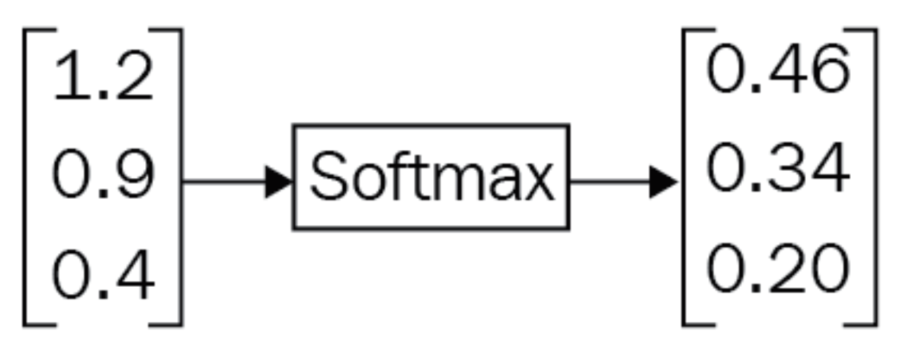
\includegraphics[width=0.4\textwidth]{Images/DataMining/softmax}
	\caption{Example of applying the softmax function \cite{Sewak:2018}} \label{fig:softmax}
\end{figure}


\section{Python Example Code}
\label{section:DataMiningExampleCode}

The identification of regional patterns within an image is facilitated by the convolutional layer. Following the convolutional layer, the max pooling layer is employed to diminish dimensionality. This section illustrates image classification by using a code provided by Sewak et al \cite{Sewak:2018}.

It is crucial to initially standardize all images to a uniform size. The initial convolution layer necessitates an additional parameter, \PYTHON{input.shape()}. The focus here is on training a Convolutional Neural Network (CNN) for image classification using the CIFAR-10 database. CIFAR-10 comprises 60,000 color images, each of size $32 \times 32$. These images are categorized into 10 classes, with 6,000 images per category, namely airplane, automobile, bird, cat, dog, deer, frog, horse, ship, and truck.

\subsubsection{Imports}

In the Listing \ref{code:cnnImports} are the necessary libraries and modules required for working with neural networks, image data, and visualization. The versions are shown in the Table \ref{tab:cnnlibraryVersions}.

\begin{itemize}
	\item Python version: 3.9.
\end{itemize}

\begin{table}[htbp]
	\centering
	\caption{Versions of Libraries}
	\label{tab:cnnlibraryVersions}
	\begin{tabular}{|l|c|}
		\hline
		\textbf{Library} & \textbf{Version} \\
		\hline
		Numpy & 1.23.5 \\
		Matplotlib & 3.7.1 \\
		Keras & 2.12.0 \\
		\hline
	\end{tabular}
\end{table}

\begin{code}[h!]
	\lstinputlisting[language=Python, numbers=none, linerange={82-89}]{Code/CNN/CNNDataMining.py}    
	
	\caption{Importing necessary libraries and modules.}
	\label{code:cnnImports}
\end{code}

\subsubsection{Load CIFAR-10 Dataset}

In Listing \ref{code:cnnLoadCifar} the CIFAR-10 dataset is loaded.CIFAR-10 is a dataset of 50,000 $32 \times 32$ color training images and 10,000 test images.

\begin{code}[h!]
	\lstinputlisting[language=Python, numbers=none, linerange={107-107}]{Code/CNN/CNNDataMining.py}    
	
	\caption{Loading and preparing the CIFAR-10 dataset.}
	\label{code:cnnLoadCifar}
\end{code}

\subsubsection{Data Preprocessing}

In the Listing \ref{code:cnnDataPreprocessing} the image data is normalized and one-hot encoding is performed on the labels. The training set is split into training and validation sets.

\begin{code}[h!]
	\lstinputlisting[language=Python, numbers=none, linerange={124-133}]{Code/CNN/CNNDataMining.py}    
	
	\caption{Preprocessing data: normalization, one-hot encoding, and splitting into training and validation sets}
	\label{code:cnnDataPreprocessing}
\end{code}

\subsubsection{Augmented Image Generator}

In the Listing \ref{code:cnnAugmentedGenerator} image data generators for training and validation is created and configured. These generators will perform data augmentation, such as shifting and flipping, to increase the diversity of the training set.

\begin{code}[h!]
	\lstinputlisting[language=Python, numbers=none, linerange={154-168}]{Code/CNN/CNNDataMining.py}    
	
	\caption{Configuring image data generators for augmentation and fitting them on training and validation data}
	\label{code:cnnAugmentedGenerator}
\end{code}

\subsubsection{Plot the First Nine Images of Cifar-10}

Listing \ref{code:cnnPlotCifar10} loads the cifar-10 dataset and plots the first nine images as shown in Figure \ref{fig:cnnFirstNineCifar10}.

\begin{code}[h!]
	\lstinputlisting[language=Python, numbers=none, linerange={177-183}]{Code/CNN/CNNDataMining.py}    
	
	\caption{Loading and visualizing the first nine images from the CIFAR-10 dataset}
	\label{code:cnnPlotCifar10}
\end{code}

\begin{figure}[h!]
	\centering
	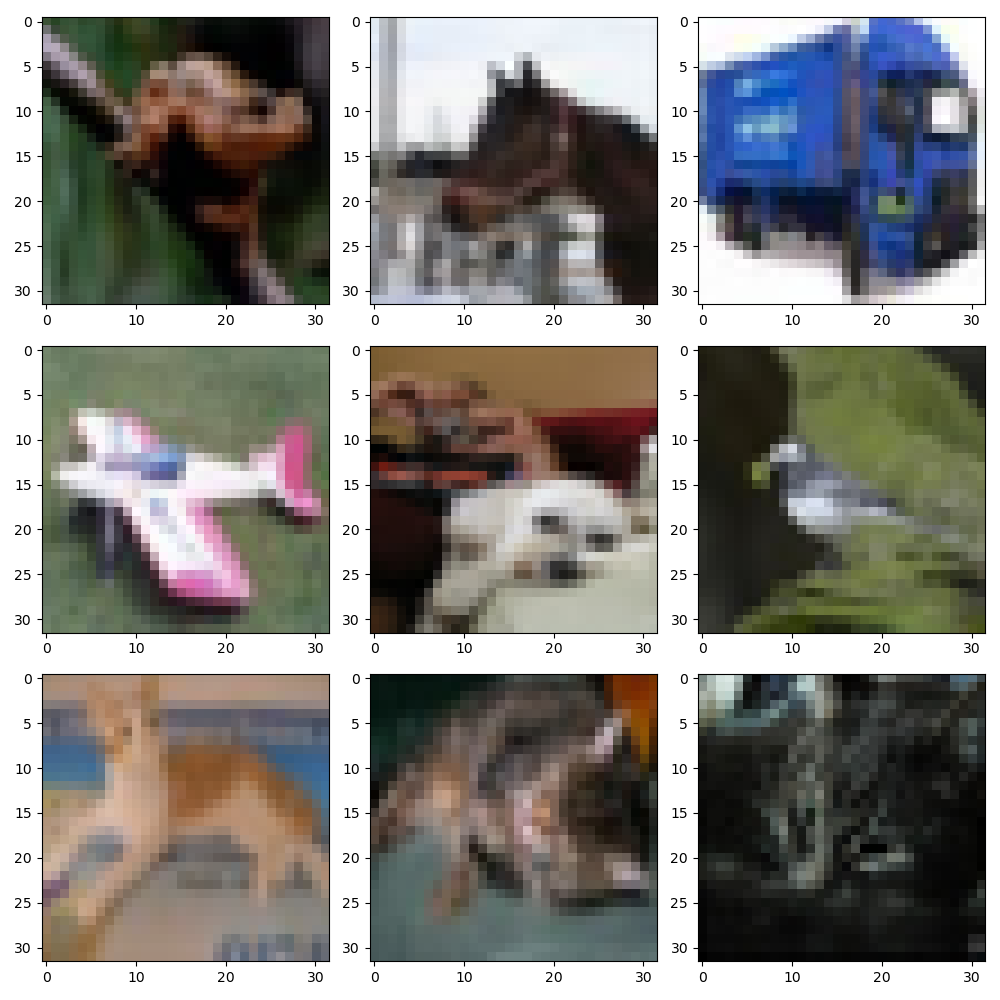
\includegraphics[width=0.8\textwidth]{Images/DataMining/CIFAR10FirstNineImages}
	\caption{First nine images from the CIFAR-10 dataset.} \label{fig:cnnFirstNineCifar10}
\end{figure}

\subsubsection{CNN Model Definition}

A Convolutional Neural Network (CNN) model is defined in Listing \ref{code:cnnDefinition} using Keras with convolutional layers, max pooling, dropout for regularization, and dense layers.

\begin{code}[h!]
	\lstinputlisting[language=Python, numbers=none, linerange={199-207}]{Code/CNN/CNNDataMining.py}    
	
	\caption{Defining a Convolutional Neural Network (CNN) model using Keras}
	\label{code:cnnDefinition}
\end{code}

\subsubsection{Compile the Model}

In Listing \ref{code:cnnCompileModel} the model is compiled with the specified loss function, optimizer, and evaluation metric.

\begin{code}[h!]
	\lstinputlisting[language=Python, numbers=none, linerange={223-223}]{Code/CNN/CNNDataMining.py}    
	
	\caption{Compiling the CNN model with specified loss function, optimizer, and metric}
	\label{code:cnnCompileModel}
\end{code}

\subsubsection{Train the Model with Augmented Data}

In Listing \ref{code:cnnTrainAugmented} the model is trained using the augmented data generators. This involves calling the \PYTHON{fit\_generator} function instead of \PYTHON{fit} and providing the data generators for training and validation sets.

\begin{code}[h!]
	\lstinputlisting[language=Python, numbers=none, linerange={238-247}]{Code/CNN/CNNDataMining.py}    
	
	\caption{Training the CNN model with augmented data using data generators}
	\label{code:cnnTrainAugmented}
\end{code}

\subsubsection{Plotting the Loss and Accuracy Curves}

In Listing \ref{code:cnnLossAccuracyPlot} the accuracy and loss curves are plotted. The results are shown in the Figure \ref{fig:AccuracyandLoss}. The observed trends in the training and validation metrics, with a downward trend in both training and validation loss and an upward trend in accuracy, indicate positive learning and generalization behavior of the neural network. The somewhat unconventional scenario of validation loss being below training loss and validation accuracy exceeding training accuracy could be influenced by effective data augmentation, contributing to the model's robustness. These trends collectively suggest that the model is not overfitting the training data and is likely to generalize well to unseen data, highlighting successful training and potential for further improvement.

\begin{code}[h!]
	\lstinputlisting[language=Python, numbers=none, linerange={263-284}]{Code/CNN/CNNDataMining.py}    
	
	\caption{Plotting the loss and accuracy curves}
	\label{code:cnnLossAccuracyPlot}
\end{code}

\begin{figure}[h!]
	\centering
	
	\begin{subfigure}{0.45\textwidth}
		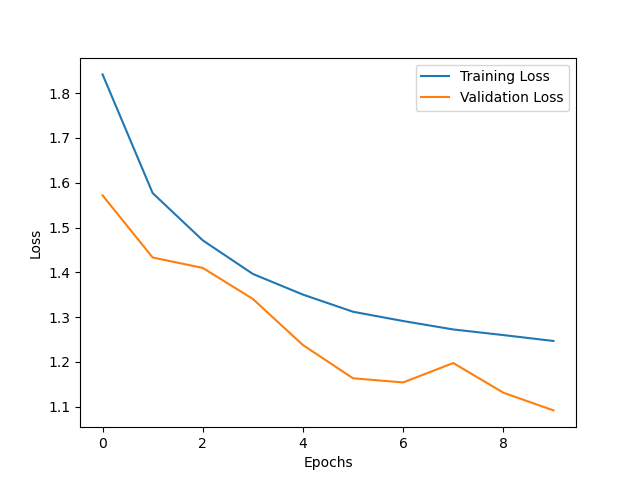
\includegraphics[width=\linewidth]{Images/DataMining/lossPlot}
		\caption{}    % \caption{} is kept to keep (a), (b), (c) etc. below each subfigure.
		\label{subfig:lossTrends}
	\end{subfigure}
	\hfill
	\begin{subfigure}{0.45\textwidth}
		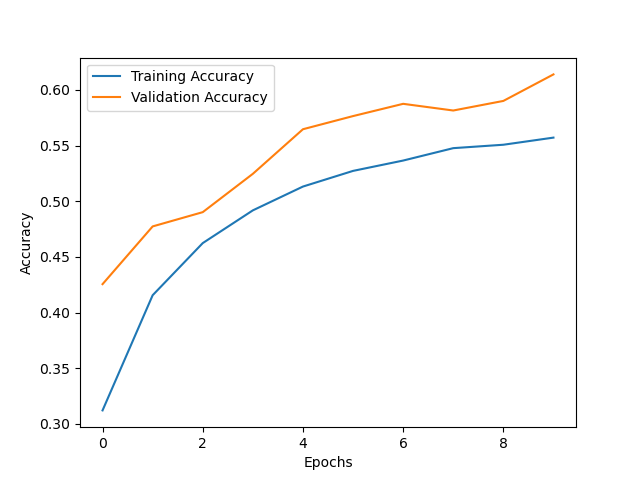
\includegraphics[width=\linewidth]{Images/DataMining/accuracyPlot}
		\caption{}    % \caption{} is kept to keep (a), (b), (c) etc. below each subfigure.
		\label{subfig:accuracyTrends}
	\end{subfigure}
	
	\caption{(\subref{subfig:DigitalImage}) Training and validation loss trends over epochs. (\subref{subfig:DigitalImagePixelValues}) Training and validation accuracy trends over epochs.}
	\label{fig:AccuracyandLoss}
\end{figure}


\section{Conclusion}

The Convolutional Neural Network (CNN) algorithm stands out as a powerful and versatile tool in the field of image processing and pattern recognition. Through its unique architecture, which includes convolutional layers for feature extraction and pooling layers for spatial down-sampling, CNNs have demonstrated remarkable success in tasks such as image classification, object detection, and facial recognition.

The effectiveness of a CNN is intricately tied to the quality and representativeness of its training data. If the dataset used for training is flawed, biased, or insufficient, the network is likely to learn and perpetuate those shortcomings, leading to suboptimal performance in real-world applications. This principle underscores the critical importance of meticulous data curation, ensuring that the input data is not only abundant but also diverse, accurate, and devoid of biases. 
Taking into account domain knowledge is crucial to avoid the "garbage in, garbage out" pitfall when engaged in the application of machine learning algorithms, as depicted in the Figure \ref{fig:DataScienceVenn}.

\begin{figure}[h!]
	\centering
	%%%%%%%%%%%%%%%%%%%%%%%%
%
% $Author: Sadegh Naderi $
% $Datum: 24.08.2023  $
% $Pfad: ML23-01-Keyword-Spotting-with-an-Arduino-Nano-33-BLE-Sense\report\Images\DataMining\DataScienceVenn.tex $
% $Version: 1.0 $
%
% !TeX encoding = utf8
%
%%%%%%%%%%%%%%%%%%%%%%%%


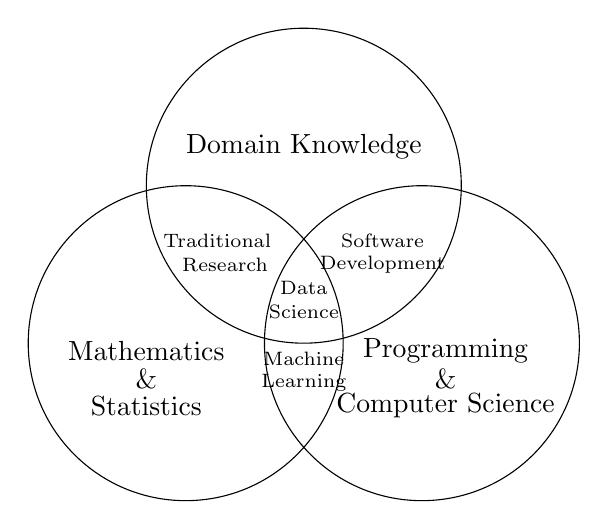
\begin{tikzpicture}
	% Mathematics & Statistics circle
	\draw (0,0) circle (2cm);
	\node at (-.5,-.1) {Mathematics};
	\node at (-.5,-.45) {\&};
	\node at (-.5,-.8) {Statistics};
	
	% Programming & Computer Science circle
	\draw (3,0) circle (2cm);
	\node at (3.3,-.1) {Programming};
	\node at (3.3,-.45) {\&};
	\node at (3.3,-.8) {Computer Science};
	
	% Domain Knowledge circle
	\draw (1.5,2) circle (2cm);
	\node at (1.5,2.5) {Domain Knowledge};
	
	% Intersection labels
	\node at (0.4,1.3) {\scriptsize{Traditional}};
	\node at (0.5,1) {\scriptsize{Research}};
	\node at (2.5,1.3) {\scriptsize{Software}};
	\node at (2.5,1) {\scriptsize{Development}};
	\node at (1.5,.7) {\scriptsize{Data}};
	\node at (1.5,0.4) {\scriptsize{Science}};
	\node at (1.5,-.2) {\scriptsize{Machine}};
	\node at (1.5,-0.5) {\scriptsize{Learning}};
	
\end{tikzpicture}

	\caption{Key areas of expertise, data science venn diagram} \label{fig:DataScienceVenn}
\end{figure}

